% Options for packages loaded elsewhere
\PassOptionsToPackage{unicode}{hyperref}
\PassOptionsToPackage{hyphens}{url}
%
\documentclass[
  ignorenonframetext,
]{beamer}
\usepackage{pgfpages}
\setbeamertemplate{caption}[numbered]
\setbeamertemplate{caption label separator}{: }
\setbeamercolor{caption name}{fg=normal text.fg}
\beamertemplatenavigationsymbolsempty
% Prevent slide breaks in the middle of a paragraph
\widowpenalties 1 10000
\raggedbottom
\setbeamertemplate{part page}{
  \centering
  \begin{beamercolorbox}[sep=16pt,center]{part title}
    \usebeamerfont{part title}\insertpart\par
  \end{beamercolorbox}
}
\setbeamertemplate{section page}{
  \centering
  \begin{beamercolorbox}[sep=12pt,center]{part title}
    \usebeamerfont{section title}\insertsection\par
  \end{beamercolorbox}
}
\setbeamertemplate{subsection page}{
  \centering
  \begin{beamercolorbox}[sep=8pt,center]{part title}
    \usebeamerfont{subsection title}\insertsubsection\par
  \end{beamercolorbox}
}
\AtBeginPart{
  \frame{\partpage}
}
\AtBeginSection{
  \ifbibliography
  \else
    \frame{\sectionpage}
  \fi
}
\AtBeginSubsection{
  \frame{\subsectionpage}
}
\usepackage{lmodern}
\usepackage{amssymb,amsmath}
\usepackage{ifxetex,ifluatex}
\ifnum 0\ifxetex 1\fi\ifluatex 1\fi=0 % if pdftex
  \usepackage[T1]{fontenc}
  \usepackage[utf8]{inputenc}
  \usepackage{textcomp} % provide euro and other symbols
\else % if luatex or xetex
  \usepackage{unicode-math}
  \defaultfontfeatures{Scale=MatchLowercase}
  \defaultfontfeatures[\rmfamily]{Ligatures=TeX,Scale=1}
\fi
% Use upquote if available, for straight quotes in verbatim environments
\IfFileExists{upquote.sty}{\usepackage{upquote}}{}
\IfFileExists{microtype.sty}{% use microtype if available
  \usepackage[]{microtype}
  \UseMicrotypeSet[protrusion]{basicmath} % disable protrusion for tt fonts
}{}
\makeatletter
\@ifundefined{KOMAClassName}{% if non-KOMA class
  \IfFileExists{parskip.sty}{%
    \usepackage{parskip}
  }{% else
    \setlength{\parindent}{0pt}
    \setlength{\parskip}{6pt plus 2pt minus 1pt}}
}{% if KOMA class
  \KOMAoptions{parskip=half}}
\makeatother
\usepackage{xcolor}
\IfFileExists{xurl.sty}{\usepackage{xurl}}{} % add URL line breaks if available
\IfFileExists{bookmark.sty}{\usepackage{bookmark}}{\usepackage{hyperref}}
\hypersetup{
  pdftitle={Introduction to R and the tidyverse},
  pdfauthor={Paolo Crosetto},
  hidelinks,
  pdfcreator={LaTeX via pandoc}}
\urlstyle{same} % disable monospaced font for URLs
\newif\ifbibliography
\usepackage{color}
\usepackage{fancyvrb}
\newcommand{\VerbBar}{|}
\newcommand{\VERB}{\Verb[commandchars=\\\{\}]}
\DefineVerbatimEnvironment{Highlighting}{Verbatim}{commandchars=\\\{\}}
% Add ',fontsize=\small' for more characters per line
\usepackage{framed}
\definecolor{shadecolor}{RGB}{248,248,248}
\newenvironment{Shaded}{\begin{snugshade}}{\end{snugshade}}
\newcommand{\AlertTok}[1]{\textcolor[rgb]{0.94,0.16,0.16}{#1}}
\newcommand{\AnnotationTok}[1]{\textcolor[rgb]{0.56,0.35,0.01}{\textbf{\textit{#1}}}}
\newcommand{\AttributeTok}[1]{\textcolor[rgb]{0.77,0.63,0.00}{#1}}
\newcommand{\BaseNTok}[1]{\textcolor[rgb]{0.00,0.00,0.81}{#1}}
\newcommand{\BuiltInTok}[1]{#1}
\newcommand{\CharTok}[1]{\textcolor[rgb]{0.31,0.60,0.02}{#1}}
\newcommand{\CommentTok}[1]{\textcolor[rgb]{0.56,0.35,0.01}{\textit{#1}}}
\newcommand{\CommentVarTok}[1]{\textcolor[rgb]{0.56,0.35,0.01}{\textbf{\textit{#1}}}}
\newcommand{\ConstantTok}[1]{\textcolor[rgb]{0.00,0.00,0.00}{#1}}
\newcommand{\ControlFlowTok}[1]{\textcolor[rgb]{0.13,0.29,0.53}{\textbf{#1}}}
\newcommand{\DataTypeTok}[1]{\textcolor[rgb]{0.13,0.29,0.53}{#1}}
\newcommand{\DecValTok}[1]{\textcolor[rgb]{0.00,0.00,0.81}{#1}}
\newcommand{\DocumentationTok}[1]{\textcolor[rgb]{0.56,0.35,0.01}{\textbf{\textit{#1}}}}
\newcommand{\ErrorTok}[1]{\textcolor[rgb]{0.64,0.00,0.00}{\textbf{#1}}}
\newcommand{\ExtensionTok}[1]{#1}
\newcommand{\FloatTok}[1]{\textcolor[rgb]{0.00,0.00,0.81}{#1}}
\newcommand{\FunctionTok}[1]{\textcolor[rgb]{0.00,0.00,0.00}{#1}}
\newcommand{\ImportTok}[1]{#1}
\newcommand{\InformationTok}[1]{\textcolor[rgb]{0.56,0.35,0.01}{\textbf{\textit{#1}}}}
\newcommand{\KeywordTok}[1]{\textcolor[rgb]{0.13,0.29,0.53}{\textbf{#1}}}
\newcommand{\NormalTok}[1]{#1}
\newcommand{\OperatorTok}[1]{\textcolor[rgb]{0.81,0.36,0.00}{\textbf{#1}}}
\newcommand{\OtherTok}[1]{\textcolor[rgb]{0.56,0.35,0.01}{#1}}
\newcommand{\PreprocessorTok}[1]{\textcolor[rgb]{0.56,0.35,0.01}{\textit{#1}}}
\newcommand{\RegionMarkerTok}[1]{#1}
\newcommand{\SpecialCharTok}[1]{\textcolor[rgb]{0.00,0.00,0.00}{#1}}
\newcommand{\SpecialStringTok}[1]{\textcolor[rgb]{0.31,0.60,0.02}{#1}}
\newcommand{\StringTok}[1]{\textcolor[rgb]{0.31,0.60,0.02}{#1}}
\newcommand{\VariableTok}[1]{\textcolor[rgb]{0.00,0.00,0.00}{#1}}
\newcommand{\VerbatimStringTok}[1]{\textcolor[rgb]{0.31,0.60,0.02}{#1}}
\newcommand{\WarningTok}[1]{\textcolor[rgb]{0.56,0.35,0.01}{\textbf{\textit{#1}}}}
\usepackage{graphicx,grffile}
\makeatletter
\def\maxwidth{\ifdim\Gin@nat@width>\linewidth\linewidth\else\Gin@nat@width\fi}
\def\maxheight{\ifdim\Gin@nat@height>\textheight\textheight\else\Gin@nat@height\fi}
\makeatother
% Scale images if necessary, so that they will not overflow the page
% margins by default, and it is still possible to overwrite the defaults
% using explicit options in \includegraphics[width, height, ...]{}
\setkeys{Gin}{width=\maxwidth,height=\maxheight,keepaspectratio}
% Set default figure placement to htbp
\makeatletter
\def\fps@figure{htbp}
\makeatother
\setlength{\emergencystretch}{3em} % prevent overfull lines
\providecommand{\tightlist}{%
  \setlength{\itemsep}{0pt}\setlength{\parskip}{0pt}}
\setcounter{secnumdepth}{-\maxdimen} % remove section numbering

\title{Introduction to R and the tidyverse}
\author{Paolo Crosetto}
\date{}

\begin{document}
\frame{\titlepage}

\hypertarget{lecture-1-plotting}{%
\section{Lecture 1: plotting}\label{lecture-1-plotting}}

\begin{frame}{Before we start: Rstudio}
\protect\hypertarget{before-we-start-rstudio}{}

\begin{itemize}
\tightlist
\item
  Interactive console
\item
  Object explorer
\item
  Script window
\item
  Plot window
\end{itemize}

\end{frame}

\begin{frame}{Before we start: R}
\protect\hypertarget{before-we-start-r}{}

\begin{itemize}
\tightlist
\item
  concatenate: c()
\item
  assign: \textless-
\item
  vector, matrices: rbind(), cbind()
\item
  matrix extraction: {[} {]}
\item
  variable extraction: \$
\item
  data frames: mpg
\end{itemize}

\end{frame}

\begin{frame}{Why do we plot}
\protect\hypertarget{why-do-we-plot}{}

\begin{quote}
\emph{Why do we want to plot data?}
\end{quote}

\begin{itemize}
\tightlist
\item
  we are human beings -- we are pattern recognizers
\item
  we can \emph{see} things we are not able to grasp from data
\item
  good to explore a dataset and look for regularities
\item
  good to \emph{convey a clear message}
\item
  to have fun
\item
  (to show your colleagues how nice your plot is)
\end{itemize}

\end{frame}

\begin{frame}{What do you see?}
\protect\hypertarget{what-do-you-see}{}

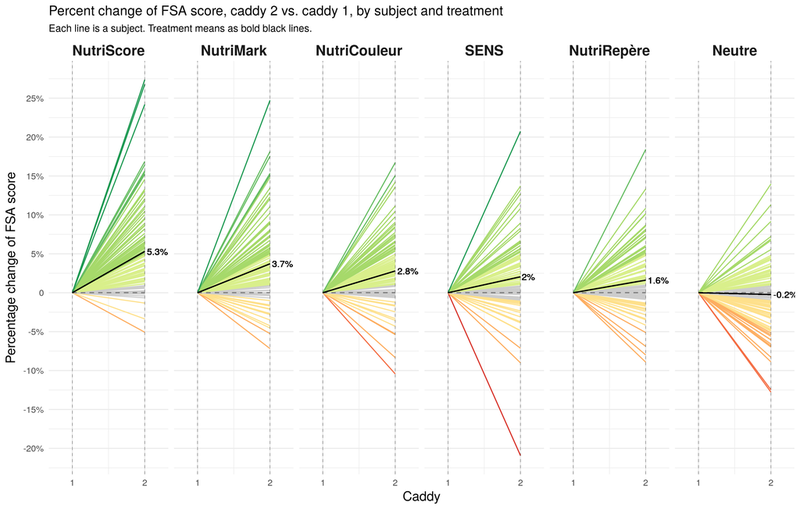
\includegraphics{fig/SlopePlot_pourcentage.png}

\begin{itemize}
\tightlist
\item
  Plots allow to convey a lot of information in a compact way
\end{itemize}

\end{frame}

\begin{frame}{Good plots, bad plots}
\protect\hypertarget{good-plots-bad-plots}{}

\begin{itemize}
\item
  It is important to make \emph{good} plots
\item
  i.e., plots that \emph{look good}\ldots{}
\item
  \ldots and are \emph{honest} to the data
\item
  it is very easy to \emph{hide} the message rather than
  \emph{highlighting} it
\item
  it is very easy to \emph{mislead} with a plot
\item
  so let's start with a gallery of \textbf{bad plots}. Can you guess
  \emph{why} they are bad?
\end{itemize}

\end{frame}

\begin{frame}{Bad plotting 1}
\protect\hypertarget{bad-plotting-1}{}

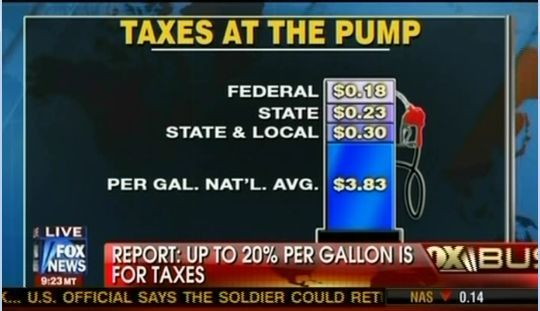
\includegraphics{fig/bad_scale_axis.jpg}

\end{frame}

\begin{frame}{Bad plotting 2}
\protect\hypertarget{bad-plotting-2}{}

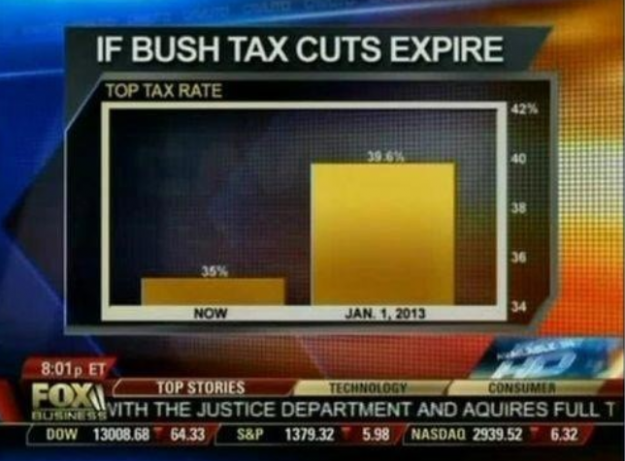
\includegraphics{fig/bar_comparison.png}

\end{frame}

\begin{frame}{Bad plotting 3}
\protect\hypertarget{bad-plotting-3}{}

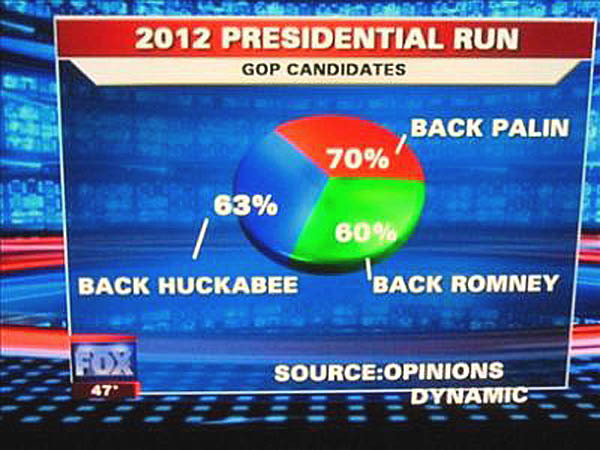
\includegraphics{fig/bad_scale_100_pie.jpg}

\end{frame}

\begin{frame}{Bad plotting 4}
\protect\hypertarget{bad-plotting-4}{}

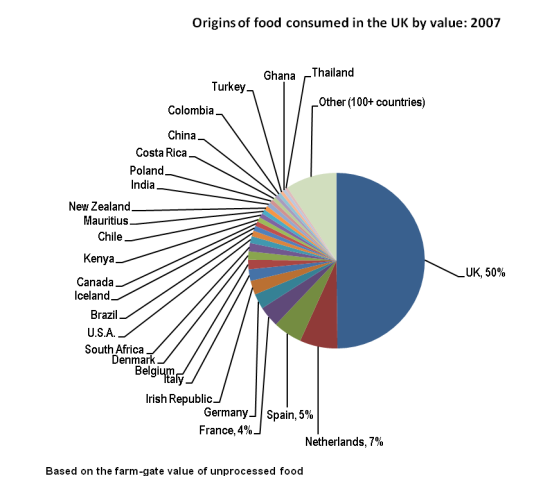
\includegraphics{fig/toomuchtext.PNG}

\end{frame}

\begin{frame}{Bad plotting 5}
\protect\hypertarget{bad-plotting-5}{}

\includegraphics{fig/3d_1st.gif}

\end{frame}

\begin{frame}{Bad plotting 5 (really, you don't need 3D plots)}
\protect\hypertarget{bad-plotting-5-really-you-dont-need-3d-plots}{}

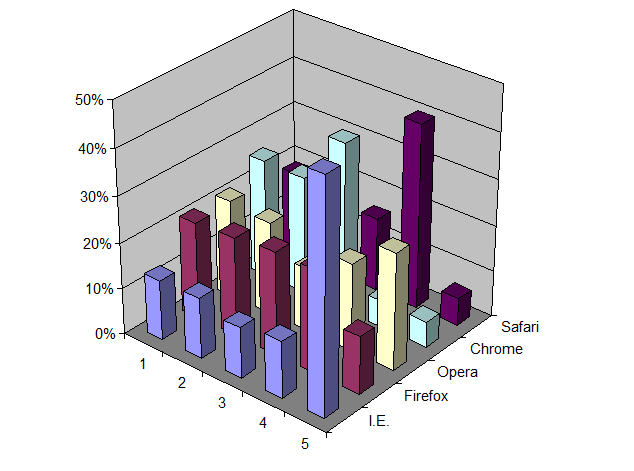
\includegraphics{fig/3d_2nd.png}

\end{frame}

\begin{frame}{The road to good plotting}
\protect\hypertarget{the-road-to-good-plotting}{}

\begin{itemize}
\tightlist
\item
  know your data
\item
  think before you hit the enter button
\item
  sketch on paper first
\item
  be honest
\item
  draw your axis first
\item
  choose your visualization wisely
\end{itemize}

\end{frame}

\begin{frame}[fragile]{Some data}
\protect\hypertarget{some-data}{}

We will start by using the \emph{built-in dataset} \textbf{mpg}

\begin{Shaded}
\begin{Highlighting}[]
\NormalTok{mpg}
\end{Highlighting}
\end{Shaded}

\begin{verbatim}
## # A tibble: 234 x 11
##    manufacturer model displ  year   cyl trans drv     cty   hwy fl    class
##    <chr>        <chr> <dbl> <int> <int> <chr> <chr> <int> <int> <chr> <chr>
##  1 audi         a4      1.8  1999     4 auto~ f        18    29 p     comp~
##  2 audi         a4      1.8  1999     4 manu~ f        21    29 p     comp~
##  3 audi         a4      2    2008     4 manu~ f        20    31 p     comp~
##  4 audi         a4      2    2008     4 auto~ f        21    30 p     comp~
##  5 audi         a4      2.8  1999     6 auto~ f        16    26 p     comp~
##  6 audi         a4      2.8  1999     6 manu~ f        18    26 p     comp~
##  7 audi         a4      3.1  2008     6 auto~ f        18    27 p     comp~
##  8 audi         a4 q~   1.8  1999     4 manu~ 4        18    26 p     comp~
##  9 audi         a4 q~   1.8  1999     4 auto~ 4        16    25 p     comp~
## 10 audi         a4 q~   2    2008     4 manu~ 4        20    28 p     comp~
## # ... with 224 more rows
\end{verbatim}

\end{frame}

\begin{frame}{A look at the data}
\protect\hypertarget{a-look-at-the-data}{}

\begin{itemize}
\tightlist
\item
  \emph{model} : model name
\item
  \emph{displ} : engine displacement, in litres
\item
  \emph{year} : year of manufacture
\item
  \emph{cyl} : number of cylinders
\item
  \emph{trans} : type of transmission
\item
  \emph{drv} : f = front-wheel drive, r = rear wheel drive, 4 = 4wd
\item
  \emph{cty} : city miles per gallon
\item
  \emph{hwy} : highway miles per gallon
\item
  \emph{fl} : fuel type
\item
  \emph{class} : ``type'' of car
\end{itemize}

\end{frame}

\begin{frame}[fragile]{We will be using \texttt{ggplot2}. Why?}
\protect\hypertarget{we-will-be-using-ggplot2.-why}{}

Advantages of ggplot2

\begin{itemize}
\tightlist
\item
  consistent underlying \texttt{grammar\ of\ graphics} (Wilkinson, 2005)
\item
  plot specification at a high level of abstraction
\item
  very flexible
\item
  theme system for polishing plot appearance
\item
  mature and complete graphics system
\item
  many users, active mailing list
\end{itemize}

\end{frame}

\begin{frame}{What is a grammar of graphics?}
\protect\hypertarget{what-is-a-grammar-of-graphics}{}

The basic idea: independently specify plot building blocks and combine
them to create just about any kind of graphical display you want.
Building blocks of a graph include:

\begin{itemize}
\tightlist
\item
  data
\item
  aesthetic mapping
\item
  geometric object
\item
  statistical transformations
\item
  scales
\item
  coordinate system
\item
  position adjustments
\item
  faceting
\end{itemize}

\end{frame}

\begin{frame}[fragile]{Starting from the basics}
\protect\hypertarget{starting-from-the-basics}{}

\textbf{As in a grammar the minimal sentence is a subject in a plot the
minimal object is data }

\begin{Shaded}
\begin{Highlighting}[]
\NormalTok{p <-}\StringTok{ }\KeywordTok{ggplot}\NormalTok{(mpg)}
\end{Highlighting}
\end{Shaded}

\textbf{In a grammar, you need a verb. In plots, this is axis}

\begin{Shaded}
\begin{Highlighting}[]
\NormalTok{p <-}\StringTok{ }\KeywordTok{ggplot}\NormalTok{(mpg, }\KeywordTok{aes}\NormalTok{(}\DataTypeTok{x =}\NormalTok{ displ, }\DataTypeTok{y =}\NormalTok{ hwy))}
\end{Highlighting}
\end{Shaded}

\begin{block}{Still no plot generated!}

\end{block}

\end{frame}

\begin{frame}[fragile]{Generating a plot}
\protect\hypertarget{generating-a-plot}{}

\textbf{But you also need an object. In ggplot, this is \emph{geoms} }

\begin{Shaded}
\begin{Highlighting}[]
\NormalTok{p }\OperatorTok{+}\StringTok{ }\KeywordTok{geom_point}\NormalTok{()}
\end{Highlighting}
\end{Shaded}

\includegraphics{2_plotting_base_files/figure-beamer/unnamed-chunk-4-1.pdf}

\end{frame}

\begin{frame}[fragile]{Generating a plot, 2}
\protect\hypertarget{generating-a-plot-2}{}

\textbf{But you also need an object. In ggplot, this is \emph{geoms} }

\begin{Shaded}
\begin{Highlighting}[]
\NormalTok{p }\OperatorTok{+}\StringTok{ }\KeywordTok{geom_smooth}\NormalTok{()}
\end{Highlighting}
\end{Shaded}

\begin{verbatim}
## `geom_smooth()` using method = 'loess' and formula 'y ~ x'
\end{verbatim}

\includegraphics{2_plotting_base_files/figure-beamer/unnamed-chunk-5-1.pdf}

\end{frame}

\begin{frame}[fragile]{Generating a plot, 3}
\protect\hypertarget{generating-a-plot-3}{}

\textbf{But you also need an object. In ggplot, this is \emph{geoms} }

\begin{Shaded}
\begin{Highlighting}[]
\NormalTok{p }\OperatorTok{+}\StringTok{ }\KeywordTok{geom_smooth}\NormalTok{()}\OperatorTok{+}\KeywordTok{geom_point}\NormalTok{()}
\end{Highlighting}
\end{Shaded}

\begin{verbatim}
## `geom_smooth()` using method = 'loess' and formula 'y ~ x'
\end{verbatim}

\includegraphics{2_plotting_base_files/figure-beamer/unnamed-chunk-6-1.pdf}

\end{frame}

\begin{frame}[fragile]{The beauty of a grammar metaphor}
\protect\hypertarget{the-beauty-of-a-grammar-metaphor}{}

\begin{itemize}
\tightlist
\item
  once you get the main idea, adding things is easy
\item
  a plot is a sentence made with data
\item
  you add layers with \texttt{+}
\item
  as you would add words to a sentence
\item
  as in grammar you use adjectives to give more nuanced meaning, in
  plots you could use \texttt{+} to add color, fill, size, shape,
  etc\ldots{}
\end{itemize}

\end{frame}

\begin{frame}[fragile]{Adding meaning: color}
\protect\hypertarget{adding-meaning-color}{}

\begin{Shaded}
\begin{Highlighting}[]
\NormalTok{p }\OperatorTok{+}\StringTok{ }\KeywordTok{geom_point}\NormalTok{(}\KeywordTok{aes}\NormalTok{(}\DataTypeTok{color=}\NormalTok{class))}
\end{Highlighting}
\end{Shaded}

\includegraphics{2_plotting_base_files/figure-beamer/unnamed-chunk-7-1.pdf}

\end{frame}

\begin{frame}[fragile]{Adding meaning: size}
\protect\hypertarget{adding-meaning-size}{}

\begin{Shaded}
\begin{Highlighting}[]
\NormalTok{p }\OperatorTok{+}\StringTok{ }\KeywordTok{geom_point}\NormalTok{(}\KeywordTok{aes}\NormalTok{(}\DataTypeTok{size=}\NormalTok{cyl))}
\end{Highlighting}
\end{Shaded}

\includegraphics{2_plotting_base_files/figure-beamer/unnamed-chunk-8-1.pdf}

\end{frame}

\begin{frame}[fragile]{Adding meaning: color AND size}
\protect\hypertarget{adding-meaning-color-and-size}{}

\begin{Shaded}
\begin{Highlighting}[]
\NormalTok{p }\OperatorTok{+}\StringTok{ }\KeywordTok{geom_point}\NormalTok{(}\KeywordTok{aes}\NormalTok{(}\DataTypeTok{size =}\NormalTok{ cyl, }\DataTypeTok{color=}\NormalTok{class))}
\end{Highlighting}
\end{Shaded}

\includegraphics{2_plotting_base_files/figure-beamer/unnamed-chunk-9-1.pdf}

\end{frame}

\begin{frame}[fragile]{Adding meaning: shape}
\protect\hypertarget{adding-meaning-shape}{}

\begin{Shaded}
\begin{Highlighting}[]
\NormalTok{p }\OperatorTok{+}\StringTok{ }\KeywordTok{geom_point}\NormalTok{(}\KeywordTok{aes}\NormalTok{(}\DataTypeTok{shape=}\NormalTok{fl))}
\end{Highlighting}
\end{Shaded}

\includegraphics{2_plotting_base_files/figure-beamer/unnamed-chunk-10-1.pdf}

\end{frame}

\begin{frame}[fragile]{Adding meaning: all together}
\protect\hypertarget{adding-meaning-all-together}{}

\begin{Shaded}
\begin{Highlighting}[]
\NormalTok{p }\OperatorTok{+}\StringTok{ }\KeywordTok{geom_point}\NormalTok{(}\KeywordTok{aes}\NormalTok{(}\DataTypeTok{color=}\NormalTok{manufacturer, }\DataTypeTok{shape =}\NormalTok{fl, }\DataTypeTok{size =}\NormalTok{ cyl))}
\end{Highlighting}
\end{Shaded}

\includegraphics{2_plotting_base_files/figure-beamer/unnamed-chunk-11-1.pdf}

\end{frame}

\begin{frame}{Facets}
\protect\hypertarget{facets}{}

\begin{itemize}
\tightlist
\item
  sometimes sentences become a bit too long
\item
  it is useful to split them up in shorter sentences
\item
  for instance, you could first talk about a car, \emph{then} another
  one
\item
  in plots, you can split up the plot along a variable
\item
  so that one plot is drawn for each level of a given variable, say type
  of fuel
\end{itemize}

\end{frame}

\begin{frame}[fragile]{Facets}
\protect\hypertarget{facets-1}{}

\begin{Shaded}
\begin{Highlighting}[]
\NormalTok{p }\OperatorTok{+}\StringTok{ }\KeywordTok{geom_point}\NormalTok{(}\KeywordTok{aes}\NormalTok{(}\DataTypeTok{color=}\NormalTok{manufacturer, }\DataTypeTok{size =}\NormalTok{ cyl))}\OperatorTok{+}\KeywordTok{facet_grid}\NormalTok{(.}\OperatorTok{~}\NormalTok{fl)}
\end{Highlighting}
\end{Shaded}

\includegraphics{2_plotting_base_files/figure-beamer/unnamed-chunk-12-1.pdf}

\end{frame}

\begin{frame}{More details on the grammar}
\protect\hypertarget{more-details-on-the-grammar}{}

A ggplot is made up of

\begin{itemize}
\tightlist
\item
  data (subject)
\item
  axis (verb)
\item
  geoms (object)
\item
  aesthetic layers (size, fill color, shape, label, \ldots)
\item
  facets (splitting sentences)
\end{itemize}

And then you can change how things look and behave: - coordinate
functions (changing the axis appearance and type) - scale functions
(changing the appearance of the geoms) - theme functions (changing the
appearance of the plot itself)

\end{frame}

\begin{frame}{Exploring data with plots: one variable}
\protect\hypertarget{exploring-data-with-plots-one-variable}{}

\emph{Plot types depend on the variable type}

\begin{itemize}
\tightlist
\item
  \emph{one-variable plots, discrete variable}: barplot
\item
  \emph{one-variable plots, continuous variable}: distribution, density
\end{itemize}

\end{frame}

\begin{frame}[fragile]{Barplots}
\protect\hypertarget{barplots}{}

\begin{itemize}
\tightlist
\item
  let's look at the drive type of the cars: front, rear, or 4wd
\end{itemize}

\begin{Shaded}
\begin{Highlighting}[]
\NormalTok{p <-}\StringTok{ }\KeywordTok{ggplot}\NormalTok{(mpg, }\KeywordTok{aes}\NormalTok{(drv))}
\NormalTok{p }\OperatorTok{+}\StringTok{ }\KeywordTok{geom_bar}\NormalTok{()}
\end{Highlighting}
\end{Shaded}

\includegraphics{2_plotting_base_files/figure-beamer/unnamed-chunk-13-1.pdf}

\end{frame}

\begin{frame}[fragile]{Barplots}
\protect\hypertarget{barplots-1}{}

\begin{itemize}
\tightlist
\item
  not so fancy. should we add color?
\end{itemize}

\begin{Shaded}
\begin{Highlighting}[]
\NormalTok{p <-}\StringTok{ }\KeywordTok{ggplot}\NormalTok{(mpg, }\KeywordTok{aes}\NormalTok{(drv))}
\NormalTok{p }\OperatorTok{+}\StringTok{ }\KeywordTok{geom_bar}\NormalTok{(}\KeywordTok{aes}\NormalTok{(}\DataTypeTok{color=}\NormalTok{drv))}
\end{Highlighting}
\end{Shaded}

\includegraphics{2_plotting_base_files/figure-beamer/unnamed-chunk-14-1.pdf}

\end{frame}

\begin{frame}[fragile]{Barplots}
\protect\hypertarget{barplots-2}{}

\begin{itemize}
\tightlist
\item
  ups. Maybe we meant fill?
\end{itemize}

\begin{Shaded}
\begin{Highlighting}[]
\NormalTok{p <-}\StringTok{ }\KeywordTok{ggplot}\NormalTok{(mpg, }\KeywordTok{aes}\NormalTok{(drv))}
\NormalTok{p }\OperatorTok{+}\StringTok{ }\KeywordTok{geom_bar}\NormalTok{(}\KeywordTok{aes}\NormalTok{(}\DataTypeTok{fill=}\NormalTok{drv))}
\end{Highlighting}
\end{Shaded}

\includegraphics{2_plotting_base_files/figure-beamer/unnamed-chunk-15-1.pdf}

\end{frame}

\begin{frame}[fragile]{Barplots}
\protect\hypertarget{barplots-3}{}

\begin{itemize}
\tightlist
\item
  nice. doesn't add much information, though. what if we cross it with
  car class?
\end{itemize}

\begin{Shaded}
\begin{Highlighting}[]
\NormalTok{p <-}\StringTok{ }\KeywordTok{ggplot}\NormalTok{(mpg, }\KeywordTok{aes}\NormalTok{(drv))}
\NormalTok{p }\OperatorTok{+}\StringTok{ }\KeywordTok{geom_bar}\NormalTok{(}\KeywordTok{aes}\NormalTok{(}\DataTypeTok{fill=}\NormalTok{class))}
\end{Highlighting}
\end{Shaded}

\includegraphics{2_plotting_base_files/figure-beamer/unnamed-chunk-16-1.pdf}

\end{frame}

\begin{frame}[fragile]{Barplots}
\protect\hypertarget{barplots-4}{}

\begin{itemize}
\tightlist
\item
  By default stacked. How to unstack?
\end{itemize}

\begin{Shaded}
\begin{Highlighting}[]
\NormalTok{p <-}\StringTok{ }\KeywordTok{ggplot}\NormalTok{(mpg, }\KeywordTok{aes}\NormalTok{(drv))}
\NormalTok{p }\OperatorTok{+}\StringTok{ }\KeywordTok{geom_bar}\NormalTok{(}\KeywordTok{aes}\NormalTok{(}\DataTypeTok{fill=}\NormalTok{class), }\DataTypeTok{position =} \KeywordTok{position_dodge}\NormalTok{())}
\end{Highlighting}
\end{Shaded}

\includegraphics{2_plotting_base_files/figure-beamer/unnamed-chunk-17-1.pdf}

\end{frame}

\begin{frame}[fragile]{Barplots}
\protect\hypertarget{barplots-5}{}

\begin{itemize}
\tightlist
\item
  By default stacked. How to show relative weight?
\end{itemize}

\begin{Shaded}
\begin{Highlighting}[]
\NormalTok{p <-}\StringTok{ }\KeywordTok{ggplot}\NormalTok{(mpg, }\KeywordTok{aes}\NormalTok{(drv))}
\NormalTok{p }\OperatorTok{+}\StringTok{ }\KeywordTok{geom_bar}\NormalTok{(}\KeywordTok{aes}\NormalTok{(}\DataTypeTok{fill=}\NormalTok{class), }\DataTypeTok{position =} \KeywordTok{position_fill}\NormalTok{())}
\end{Highlighting}
\end{Shaded}

\includegraphics{2_plotting_base_files/figure-beamer/unnamed-chunk-18-1.pdf}

\end{frame}

\begin{frame}[fragile]{One variable, continuous: mpg on highway}
\protect\hypertarget{one-variable-continuous-mpg-on-highway}{}

\begin{itemize}
\tightlist
\item
  When the variable is continuous, it makes more sense to show
  distributions
\end{itemize}

\begin{Shaded}
\begin{Highlighting}[]
\NormalTok{p <-}\StringTok{ }\KeywordTok{ggplot}\NormalTok{(mpg, }\KeywordTok{aes}\NormalTok{(hwy))}
\NormalTok{p }\OperatorTok{+}\StringTok{ }\KeywordTok{geom_histogram}\NormalTok{()}
\end{Highlighting}
\end{Shaded}

\begin{verbatim}
## `stat_bin()` using `bins = 30`. Pick better value with `binwidth`.
\end{verbatim}

\includegraphics{2_plotting_base_files/figure-beamer/unnamed-chunk-19-1.pdf}

\end{frame}

\begin{frame}[fragile]{Histograms: binwidth}
\protect\hypertarget{histograms-binwidth}{}

\begin{Shaded}
\begin{Highlighting}[]
\NormalTok{p }\OperatorTok{+}\StringTok{ }\KeywordTok{geom_histogram}\NormalTok{(}\DataTypeTok{bins =} \DecValTok{10}\NormalTok{)}
\end{Highlighting}
\end{Shaded}

\includegraphics{2_plotting_base_files/figure-beamer/unnamed-chunk-20-1.pdf}

\end{frame}

\begin{frame}[fragile]{Histograms: binwidth}
\protect\hypertarget{histograms-binwidth-1}{}

\begin{Shaded}
\begin{Highlighting}[]
\NormalTok{p }\OperatorTok{+}\StringTok{ }\KeywordTok{geom_histogram}\NormalTok{(}\DataTypeTok{bins =} \DecValTok{100}\NormalTok{)}
\end{Highlighting}
\end{Shaded}

\includegraphics{2_plotting_base_files/figure-beamer/unnamed-chunk-21-1.pdf}

\end{frame}

\begin{frame}[fragile]{An alternative do histogram: dotplot}
\protect\hypertarget{an-alternative-do-histogram-dotplot}{}

\begin{Shaded}
\begin{Highlighting}[]
\NormalTok{p }\OperatorTok{+}\StringTok{ }\KeywordTok{geom_dotplot}\NormalTok{(}\DataTypeTok{binwidth =} \FloatTok{0.5}\NormalTok{)}
\end{Highlighting}
\end{Shaded}

\includegraphics{2_plotting_base_files/figure-beamer/unnamed-chunk-22-1.pdf}

\end{frame}

\begin{frame}[fragile]{Continuous distribution: Kernel Density
Estimation}
\protect\hypertarget{continuous-distribution-kernel-density-estimation}{}

\begin{Shaded}
\begin{Highlighting}[]
\NormalTok{p }\OperatorTok{+}\StringTok{ }\KeywordTok{geom_density}\NormalTok{()}
\end{Highlighting}
\end{Shaded}

\includegraphics{2_plotting_base_files/figure-beamer/unnamed-chunk-23-1.pdf}

\end{frame}

\begin{frame}[fragile]{Continuous distribution: Kernel Density
Estimation}
\protect\hypertarget{continuous-distribution-kernel-density-estimation-1}{}

\begin{Shaded}
\begin{Highlighting}[]
\NormalTok{p }\OperatorTok{+}\StringTok{ }\KeywordTok{geom_density}\NormalTok{(}\DataTypeTok{adjust =} \DecValTok{3}\NormalTok{)}
\end{Highlighting}
\end{Shaded}

\includegraphics{2_plotting_base_files/figure-beamer/unnamed-chunk-24-1.pdf}

\end{frame}

\begin{frame}[fragile]{Continuous distribution: Kernel Density
Estimation}
\protect\hypertarget{continuous-distribution-kernel-density-estimation-2}{}

\begin{Shaded}
\begin{Highlighting}[]
\NormalTok{p }\OperatorTok{+}\StringTok{ }\KeywordTok{geom_density}\NormalTok{(}\DataTypeTok{adjust =} \FloatTok{0.5}\NormalTok{)}
\end{Highlighting}
\end{Shaded}

\includegraphics{2_plotting_base_files/figure-beamer/unnamed-chunk-25-1.pdf}

\end{frame}

\begin{frame}{Additional resources}
\protect\hypertarget{additional-resources}{}

\begin{itemize}
\tightlist
\item
  try to look for PlotCon2016 videos, and especially
  \href{https://www.youtube.com/watch?v=RG_BKQRbJZw}{this one}
\item
  \ldots{}
\end{itemize}

\end{frame}

\end{document}
